%************************************************
\chapter{All Things Classical}\label{chap:compilers}
%************************************************

Okay, maybe not \emph{all} things classical, but some things\dots
Okay, maybe just one or two really.

In this chapter we will give a very brief overview of the components of classical computers that will be helpful to further discussions of quantum circuit compilation.
A key component to quantum circuit compilation is the word ``compilation'' and its' origins (in computing) span back to the early 1950's when electronic digital computers were in their early stages.
Understanding the historical development of compilation and its' tecniques will provide ideas and tools necessary in solving the new task of quantum circuit compilation.

This chapter is meant to provide the reader with the basics of some computing terminology and ideas.
It is by no means a complete introduction to compilers, nor computer architecture.

\section{What can a computer do?}

If you're reading this, I'm sure you can imagine something your computer is capable of.
Maybe reading this document online, sending messages/email, browsing the internet, writing documents, etc.
These are very high level operations our computer can perform, but under the hood much more primitive operations are taking place.
It is these primitive operations that we wish to understand, and will have many similarities with modern-day quantum hardware.

A simplified model of computer architecture, known as the von Neumann Architecture (\cref{fig:comparch}) shows what we now call a \ac{CPU} which is the workhorse of the computer.\footnote{At least in this \emph{very simplified} model.}

\begin{figure}[h]
    \centering
    \includestandalone[width=0.8\textwidth]{tikz/arch}
    \caption{von Neumann Architecture scheme}\label{fig:comparch}
\end{figure}

Since the \ac{CPU} is the computational piece of a computer, what can it do?
Most modern \acp{CPU} are built on the \acp{ISA} which means that the \ac{CPU} has a finite set of operations or instructions that it can perform and everything we might wish to perform on a computer, must be built up from these primitive operations.
Some examples of what these primitive operations might be are
\begin{itemize}
    \item put a value into memory,
    \item add two values in memory together and store in a new location,
    \item perform the bitwise negation on a value,
    \item compute the square root of a value.
\end{itemize}
With a set of performable operations laid out, one can then use these primitives to build up more and more complex functionality that eventually implements the things we know and love (and hate) computers for.
One thing worth mentioning here that is often glossed over in treatments of \acp{ISA} is that the instruction set must be computationally universal.\footnote{Or Turing-complete if you're computer science oriented.}
Without going too much into the weeds, we should think of computationally universal (in the classical sense) as wielding the full power of a computer, rather than only being able to do a particular type of computation.\todo{I don't like this explanation.}
Thankfully, this is relatively easy to do in the classical setting and there are even theoretical machines that use a \emph{single} operation to achieve universal computation.
\Eg{} one can achieve universal classical computation with the following instruction which implements ``subtract and branch if negative''.
\begin{lstlisting}
    Instruction subneg a, b, c
    Memory[b] = Memory[b] - Memory[a]
    if (Memory[b] < 0)
        goto c
\end{lstlisting}

While this style of architecture is great, and has worked very well, it requires the programmer to code at a very low level since the operations a \ac{CPU} performs are themselves primitive.
In order to work at a higher level of abstraction, computer scientists and programmers began to create new languages which were easier to read and write, yet could be translated into a form the brains of the computer could understand.
This would improve productivity by allowing those writing code to work at a higher level of abstraction, and bury implementation details into the code which performed the translation into the machine's instruction set.
The software responsible for translating these higher level ideas into a machines instruction set are known as \textbf{compilers}.


% With the exception of the last item, these operations are generally considered to be simple, and the latter complex.
% This has given rise to a distinction in \ac{CPU} architecture where we see \acp{CISC} and \acp{RISC}.
% The goal of the former to implement more and more complex ``primitive'' operations, while the latter leaving more work to be performed by the compiler~\cite{dragonbook}.

\section{Compilers}
In order to understand what quantum circuit compilation is all about, it is helpful to first know what compilation means, and where our classical notions of compilation come from.
To start at the very beginning, Merriam-Webster defines the word \textbf{compile} to mean~\cite{compiledef}
\begin{quote}
    to compose out of materials from other documents.
\end{quote}
We can see this definition reflected in~\citetitle{dragonbook}\footnote{Colloquially known as ``The Dragon Book'' because of the cover, and likely the most famous book on (classical) compilers. This is also where the logo of the LLVM project originates from which we will discuss in~\cref{sec:llvm}.}\graffito{
    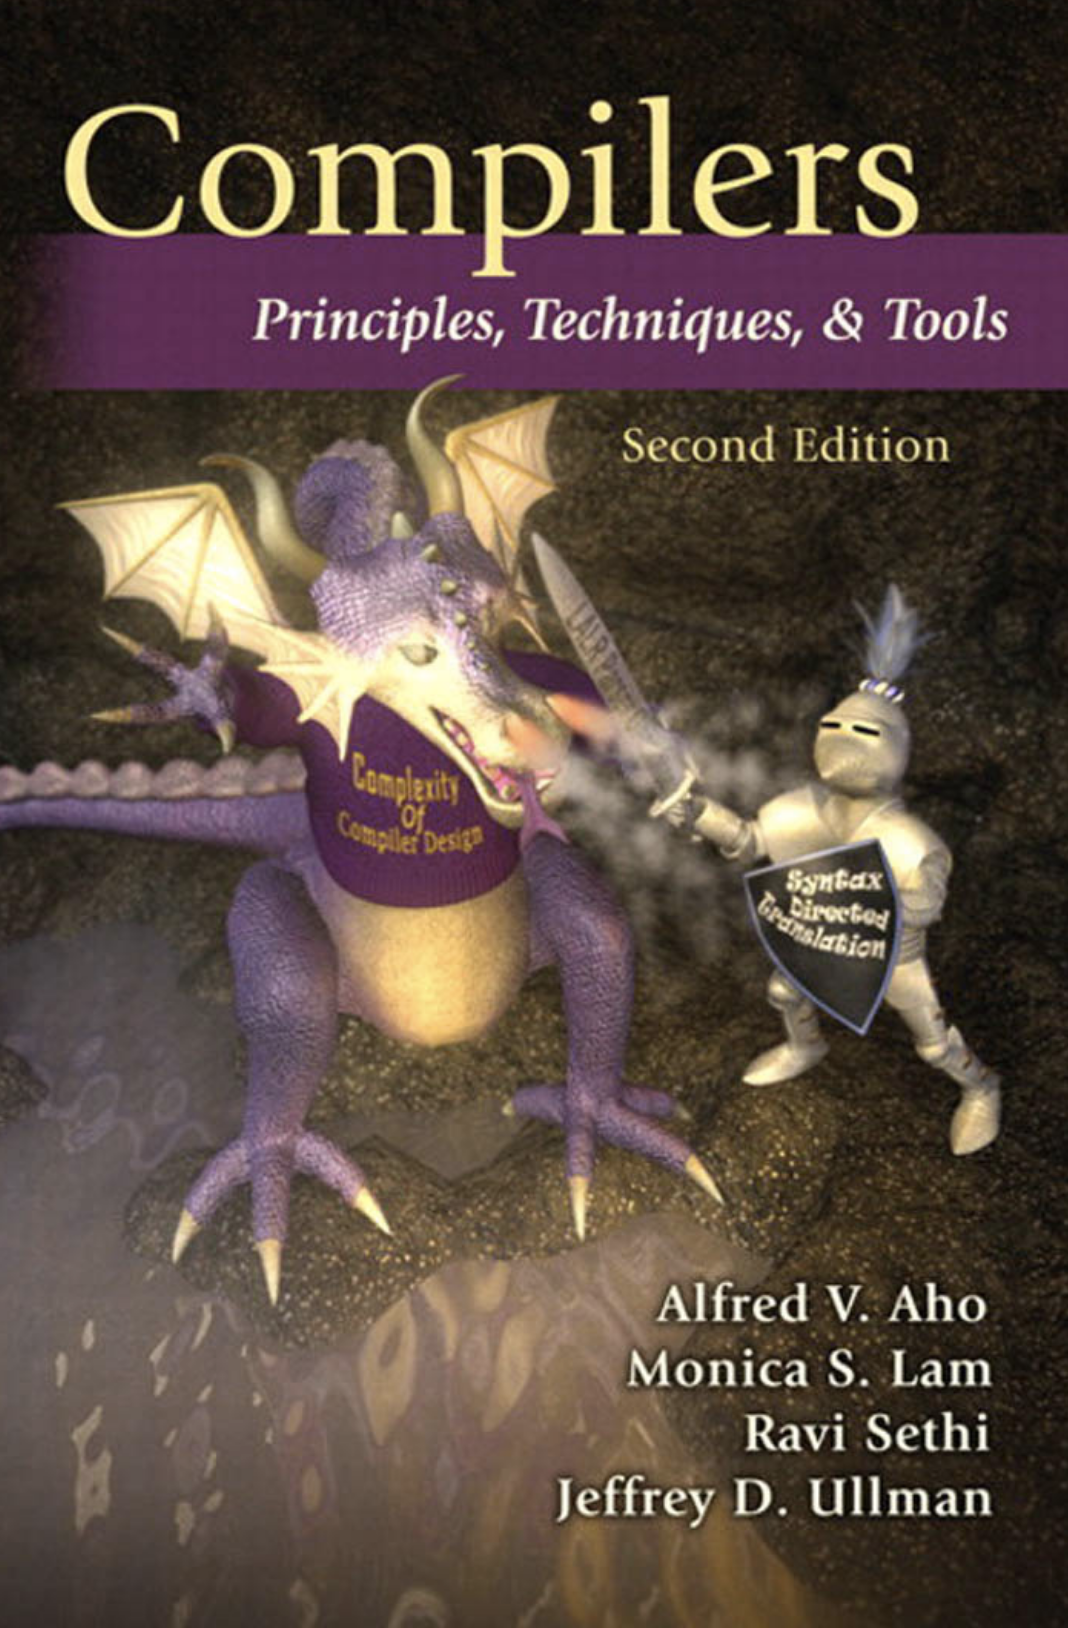
\includegraphics[width=\marginparwidth]{img/dragonbook.png}
    \emph{The Dragon Book}
    
\includegraphics[width=\marginparwidth]{img/llvmlogo.png}
    \emph{LLVM Logo}
}~\cite{dragonbook} where the authors introduce compilers through the process of transforming software.
\begin{quotation}
    [B]efore a program can be run, it first must be translated into a form in which it can be executed by a computer.

    The software systems that do this translation are called \emph{compilers}.
\end{quotation}
Hence we can visualize the action of a compiler as a sort of informal function.
\begin{figure}[ht]
    \centering
    \tikzset{
        frame/.style={
                draw,
                text width=6em,
                text centered,
                minimum height=4em,
                drop shadow,
                fill=orange!40,
                rounded corners,
            },
    }
    \begin{tikzpicture}[font=\sffamily, thick, node distance=4cm]
        \node[align=center] (pl) {Programming \\ Language};
        \node[frame, right of=pl] (compiler) {Compiler};
        \node[align=center, right of=compiler] (ml) {Machine \\ Language};

        \draw[-stealth] (pl) -- (compiler);
        \draw[-stealth] (compiler) -- (ml);
    \end{tikzpicture}
    \caption{Action of Compiler}\label{fig:compiler}
\end{figure}

The term compiler was coined by Grace Hopper in the early 1950's while working on a system that could translate symbolic mathematics into a machine language.
Initially Hopper was met with resistance for her new idea.
\begin{quotation}
    I had a running compiler, and nobody would touch it because, they carefully told me, computers could only do arithmetic; they could not do programs.
    It was a selling job to get people to try it.
    I think with any new idea, because people are allergic to change, you have to get out and sell the idea.
    \attrib{Grace Hopper 1952~\cite{hopperquote}}
\end{quotation}
In the end she succeeded in selling the idea and compilers became a ubiquitous piece of modern computing infrastructure.
Since Hopper coined the term the job of a compiler has grown enormously and now encompasses line reconstruction, preprocessing, lexical analysis, syntax analysis, semantic analysis, conversion to an \ac{IR}, optimization, target dependent optimizations, and finally code generation.
Thankfully we will not need to understand all of these parts, and the majority of this document will focus on \aclp{IR}, optimizations, and code generation.

\subsection{Examples of Compilers}
\begin{description}
    \item[Latex] While perhaps not very obvious, \LaTeX{} is indeed a compiler in the sense that it takes in code, and produces a lower level representation of what the user wants to typeset. Usually that comes in the form of postscript which is another programming language that is read by printers (hardware) to produce the requested document.
    \item[TensorFlow:] TensorFlow is a platform for machine learning that embodies the structure of a compiler very nicely. Indeed it has a front-end where the user builds their model, an optimizer that speeds up the model, and once it's ready the model can be brought to multiple backends (in browser, mobile, laptop). This is all even before we talk about TensorFlow Quantum which was introduced in~\cite{tensoflowquantum} to aid in optimizing noisy circuits on \acs{NISQ} devices.\footnote{We will get into, and define this terminology shortly!}
    \item[clang:] This \emph{is} a compiler in the strictest sense. As input it takes C/C++ and provides executable versions of that code that an be run on hardware.
\end{description}

\subsection{Intermediate Representations}

Suppose we have the following line in our code.
\begin{center}
    \verb|x_final = x_initial + velocity * time|
\end{center}
From this, one of the first steps the front end of a compiler might do is generate what's called a \textbf{syntax tree}.
This is a representation of the line of code in a tree format as in~\cref{fig:syntaxtree}.
% While it may not be obvious why this is a helpful representation, it \emph{is} indeed a representation that is used for further processing.
In this context, what we see in~\cref{fig:syntaxtree} is known as an \ac{IR} because it is not the initial, nor final representation of the piece of code.
While the compiler works with the code in this state it can perform syntactic and semantic analysis to ensure the code is well formed (syntactically), and meaningful (semantically).

Optimizations may also be performed.
\Eg{} if \verb|distance = velocity * time| has already been calculated previously in the code, the subtree
\begin{figure}[ht!]
    \centering
    \Tree [.* velocity time ]
    \caption*{}
\end{figure}
can be replaced by simply \texttt{distance}.

\begin{figure}[ht!]
    \centering
    \newcommand{\qleafhook}[1]{\texttt{#1}}
    \newcommand{\qlabelhook}[1]{\texttt{#1}}
    \Tree [.= x\_final [.+ x\_initial [.* velocity time ] ] ]
    \caption{Syntax Tree}\label{fig:syntaxtree}
\end{figure}

\subsection{Computer Architecture}
To understand why it is we need compilers in the first place, we need to understand how modern computers work.
In a highly simplified model we can think of a computer as a \ac{CPU} connected to input and output devices (think keyboard and screen), and some sort of memory.

At the very basic level, a \ac{CPU} has a finite number of possible operations it can perform despite there being a much larger input space of ``possible programs'' that we can feed it.
How then does the computer take a script and run it on it's \ac{CPU}?


Chris Lattner (the founder of one of the largest compiler projects; LLVM) has characterized compilers succinctly in~\cite{lattnerquote} as
\begin{quote}
    the art of allowing humans to think at a level of abstraction that they want to think about.
\end{quote}

\paragraph{Abstraction} With Lattner's quote in mind we can think of compilers as the tool that allows us to work with languages that are very abstract when compared to the instructions our \ac{CPU} can perform.
There also exist tools known as decompilers which take executables and turn them back into source code.
This operation is almost never the inverse of compiler because most languages allow for many ways of writing code that performs the same task.
With these tools we can raise and lower our levels of abstraction as desired and further push the details of the ``metal'' or hardware implementation away.


\section{LLVM}\label{sec:llvm}

% \subsection{\acf{MLIR}}